% ============================================================================
% APPENDICES
% ============================================================================
% 2026-10-31 (konsey turu, Y3): yeni dosya (raporlar/konsey_2026-10-29/
% 12_makale_revizyon_brifi.md Sec. 4.5). Govdeden tasinanlar:
%   Ek A app:behavior   - eski 04 Sec. G (uc okuma), epsilon taramasi, eski TGR
%                         sonucu; tanimlar eski 03 (gradyan, mekansal, dikkat,
%                         oznitelik metrikleri) kisaltilarak.
%   Ek B app:selection  - eski 04 Sec. F (secim kurali) ve Sec. H (varyans
%                         kaynaklari); subsec:selection etiketi burada korunur.
%   Ek C app:registrations - eski CIFAR-100 ve L2 kayitli ongoruleri.
% Dusenler: fig:gradient_analysis, fig:gradient_heatmap, fig:attention_layers,
% tab:tgr, tab:cifar100_results, tab:l2_results (brif Sec. 5.10, 6.9).
% tab:feature_degradation'in "All tokens" sutunu kelime butcesi icin dustu
% (foy Tablo 10'da duruyor; metin yalniz CLS ve yama ortalamasini kullanir).
% Kapi korumali ifadeler (brif Sec. 12.4): "four sources of variance",
% "$25$ epochs", "0.32", "2.85", "deliberately not as a ratio to seed-level
% dispersion" (Ek B); "0.22", "0.48", "not testable in this design",
% "we report the slope rather than a correlation" (Ek C).
% Her sayi results/C1_REFERANS_FOYU.md'den; paragraf ustunde "% FOY:" yorumu.
\appendices

\section{Behavioral Measurements of the Pair}
\label{app:behavior}

% FOY:Epsilon taramasi:356,357,358,359,360,361,362,364 (tarama), 366-370 (Tablo I ile fark)
The CNN's margin over the ViT is widest at small perturbation budgets ($77.30$ against $64.10\%$ at $2/255$) and narrows at $16/255$ ($20.38$ against $12.16\%$; Figure~\ref{fig:epsilon_sweep}).

% FOY:Epsilon taramasi:371,373 (Tablo I ile fark, 8/255)
\begin{figure}[!t]
\centering
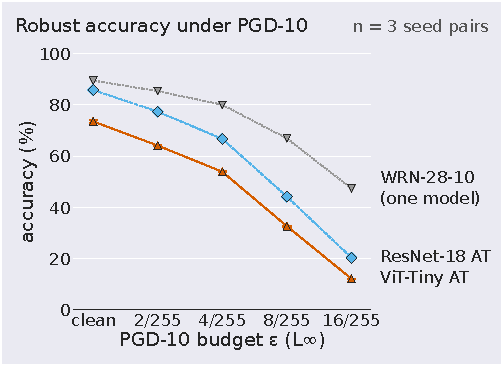
\includegraphics[width=\columnwidth]{../figures/fig16_epsilon_sweep.pdf}
\caption{\textbf{Robust accuracy under PGD-10.} Accuracy against the budget $\eps$ on the CIFAR-10 test set, mean$\pm$SD over three seed pairs with bars narrower than the markers; clean is $\eps = 0$, and WRN-28-10 is a single robust RobustBench model. This separate evaluation differs from Table~\ref{tab:main_results} by at most $0.08$ points at $8/255$.}
\label{fig:epsilon_sweep}
\end{figure}

% KAYNAK: eski 03_methodology.tex (Gradient Analysis, Spatial Locality Metrics; tanimlar)
% FOY:Gradyan yapisi:90,91,92,93,95,97,99,100,101,102 ; Tablo 8 ek sutunlari:254,262 ; M8.10:1321 (kosum basina 500 goruntu)
% FOY:M8.10:1325,1326,1327,1328,1330 ; Tablo 9 ek sutunlari:279,280,281,282
Input gradients of per-sample losses were measured on $500$ test images per run. Sparsity is scored with Hoyer sparsity, the Gini coefficient and the fraction of components below 1\% of the per-sample maximum, all scale-invariant~\cite{hurley2009comparing}, and spatial locality on the normalized channel-summed energy map (Table~\ref{tab:spatial}). CNN gradients are sparser on all three measures in every run (Table~\ref{tab:gradient}). Paired tests within runs reject the null (Holm $p \leq 2.2\times10^{-12}$), but at the run level, the unit an architectural claim needs, Holm correction leaves $p = 0.108$, so the ordering is reproducible without being significant. Adversarial training produces it: clean-trained, the ViT is the sparser model (Hoyer $0.380$ against $0.347$), and a CIFAR-native ViT is less sparse than the upsampled one. The ViT has the higher absolute alignment (run-level $p = 0.0009$), while signed alignment stays at or below $0.0014$ for both. No spatial descriptor differs at the run level (Holm $p$ from $0.40$ to $0.54$), and two of them change sign across runs, so the sparser CNN gradients are not more localized.

% FOY:Gradyan yapisi:90,91,92,93 ; Tablo 8 ek sutunlari:254,255,262,263,264,265 ; M8.10:1321 (n = 500)
\begin{table}[!t]
\centering
\caption{Gradient characteristics ($n=500$ images per run; mean$\pm$SD over three runs). The native control is one CIFAR-native ViT checkpoint (4$\times$4 patches) that predates the fixed-split protocol.}
\label{tab:gradient}
\footnotesize
\setlength{\tabcolsep}{2.5pt}
\begin{tabular}{lccc}
\toprule
\textbf{Metric} & \textbf{ResNet-18 AT} & \textbf{ViT-Tiny AT} & \textbf{ViT (native)} \\
\midrule
Hoyer sparsity & 0.4928$\pm$0.0120 & 0.4561$\pm$0.0055 & 0.4046 \\
Gini coefficient & 0.6498$\pm$0.0089 & 0.6099$\pm$0.0051 & 0.5712 \\
Fraction $<$1\% of max & 0.3477$\pm$0.0210 & 0.2682$\pm$0.0090 & 0.1785 \\
Alignment (absolute) & 0.0378$\pm$0.0009 & 0.0562$\pm$0.0004 & 0.0794 \\
Alignment (signed) & 0.0010$\pm$0.0003 & 0.0004$\pm$0.0001 & -- \\
\bottomrule
\end{tabular}
\end{table}

% FOY:C5:125,131,132,133,134 ; Tablo 9 ek sutunlari:279,280,281,282 (fark SD, Holm p)
\begin{table}[!t]
\centering
\caption{Spatial locality of input gradients ($n=500$ per run; mean$\pm$SD over three runs). $p$: one-sample $t$-test on the three per-run paired differences, Holm-corrected over the four measures.}
\label{tab:spatial}
\scriptsize
\setlength{\tabcolsep}{1.6pt}
\begin{tabular}{lcccc}
\toprule
\textbf{Measure} & \textbf{ResNet-18} & \textbf{ViT-Tiny} & \textbf{Diff.\ (R$-$V)} & \textbf{$p$ (Holm)} \\
\midrule
Area for 50\% energy & 0.0378$\pm$0.0017 & 0.0397$\pm$0.0010 & $-$0.0019$\pm$0.0027 & 0.54 \\
Area for 90\% energy & 0.2345$\pm$0.0078 & 0.2570$\pm$0.0067 & $-$0.0224$\pm$0.0133 & 0.40 \\
Spatial entropy (nat) & 5.2014$\pm$0.0387 & 5.2524$\pm$0.0197 & $-$0.0509$\pm$0.0580 & 0.54 \\
Moran's $I$ & 0.4141$\pm$0.0132 & 0.3941$\pm$0.0024 & $+$0.0200$\pm$0.0156 & 0.47 \\
\bottomrule
\end{tabular}
\end{table}

% KAYNAK: eski 03_methodology.tex (Token Aggregation, Attention Metrics, Feature Degradation Metrics)
% FOY:C4:110,111,113,120,122,123 ; Tablo 10:288-323 ; Dikkat entropisi:348,350
% FOY:Dikkat entropisi TOST:1113,1138,1139
Feature drift is the clean-to-adversarial cosine at each residual block output under the model's own PGD-10 attack ($n = 1{,}000$ per run). In the ViT it is gradual and leaves feature norms within $0.45\%$; in the CNN it concentrates in the first block of the last stage, with a cosine of $0.8777$ against $0.9607$ one block earlier and $0.9108$ one block later, and a $-13.14\pm1.89\%$ norm change. The CLS token drifts about three times as far as the patch-token mean at their minima, which lie at blocks 11 and 9. The entropy of the head-averaged CLS attention does not change: the largest per-layer change is $0.0045$ nats against clean values of $4.61$ to $5.11$, and run-level TOST at $\pm0.05$ nats accepts equivalence in all $12$ layers (top card of Figure~\ref{fig:feature_degradation}). Attention displacement grows from $0.028$ to $0.084$ with depth, so the attack redirects attention without broadening it. Last-block drift does not separate flipped from unflipped images (run-level $p = 0.20$ for the ViT, $0.080$ for the CNN).

% FOY:Dikkat entropisi TOST:1113 ; Dikkat entropisi:334-345,350
\begin{figure}[!t]
\centering
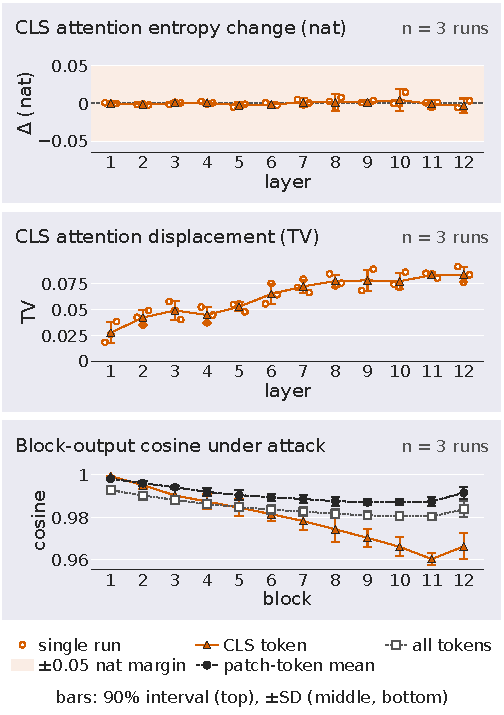
\includegraphics[width=\columnwidth]{../figures/fig17_feature_degradation.pdf}
\caption{\textbf{Feature degradation of ViT-Tiny under attack.} Per layer over three runs: CLS attention entropy change, with 90\% intervals of the run-level TOST inside the shaded $\pm0.05$-nat margin (top); CLS attention displacement (TV) (middle); Block-output cosine under attack for the CLS token, the patch-token mean and all tokens (bottom), both mean$\pm$SD. The ViT is attacked with its own PGD-10.}
\label{fig:feature_degradation}
\end{figure}

% FOY:C2:143,144,146 ; M8.4:1196 (ayri MI-FGSM kosusu, ViT->CNN 15.42)
% KAYNAK: eps 8/255, 10 adim (tasarim sabiti)
An earlier matched-budget comparison on the pair agrees with Section~\ref{subsec:attack_side}: token gradient regularization~\cite{zhang2023tgr} transferred worse than MI-FGSM~\cite{dong2018boosting} from the ViT ($12.70\pm0.41$ against $15.71\pm0.60\%$ target-correct), in a run separate from the MI-FGSM check of Section~\ref{subsec:transfer} ($15.42\pm0.52\%$).

\section{Checkpoint Selection and Sources of Variance}
\label{app:selection}
\label{subsec:selection}

% FOY:M8.7:1269,1273,1274,1286,1287,1293
Varying only how the final checkpoint is chosen from a fixed trajectory (validation split, patience and curve smoothing; eighteen combinations) moves PGD-10 accuracy by $2.62$ to $2.85$ points per seed for the ResNet and $1.58$ to $2.09$ for the ViT. This dispersion is quoted in points and deliberately not as a ratio to seed-level dispersion, because that ratio runs from $0.67$ to $3.38$ (ResNet) and $0.63$ to $7.38$ (ViT) depending on the reference cell. Selection paths can be unstable while outcomes are not: on CIFAR-100 the selected epoch varies by $25$ epochs across ResNet seeds, yet the test PGD-10 standard deviation is $0.32$ points.

% FOY:Secim kuralinin asimetriye etkisi:799,808,813,814,815,816,817,818,825 ; M8.14:1390,1392
At their last checkpoints, twenty epochs after the selected ones, the three training pairs have a clean gap of $10.55\pm0.59$ instead of $12.26\pm0.90$ points and a four-protocol spread of $12.84\pm0.34$ points, with the CNN$\rightarrow$ViT sign kept under every protocol and the identity premise intact ($p \geq 0.9915$).

% FOY:TabloI:16,17 ; TabloIII:159,160,161,162,163 ; M8.8:1295-1309
% FOY:M10.7:2049,2050 (saldiri tohumu SD'si; ilk C1 cifti 1001/2001, ilk 1000 goruntu, 3 saldiri tohumu,
% artefakt alani np.std ddof 0: CNN 0.05, ViT 0.00 puan). 2026-10-31: TODO(foy) kapandi.
The comparisons face four sources of variance. Over three attack seeds on the first $1{,}000$ test images of one seed pair, robust accuracy has a standard deviation of $0.05$ points for the CNN and $0.00$ for the ViT. Training runs move accuracy by a standard deviation of at most $0.55$ points and the transfer asymmetry by $0.23$ to $1.27$ points, depending on the protocol. Within a fixed seed pair the protocol moves the asymmetry by $15.01\pm0.84$ points, and the selection rule moves the spread by about two (Section~\ref{subsec:transfer}). The ratio of protocol to run dispersion is not used as evidence, since with two degrees of freedom its $\chi^2$ interval is very wide.

\section{Registered Predictions for CIFAR-100 and the $L_2$ Budget}
\label{app:registrations}

% FOY:TabloIII:159-163 (CIFAR-100 sutunu) ; Basarili-kaynak siki ve gevsek:240 (10.45) ; M8.2:1171
% FOY:M10.7:2058,2060,2062 (CIFAR-100 C3 hedef temiz hatalari 36.15 ve 36.36; en kucuk ara 0.21). 2026-10-31: TODO(foy) kapandi.
Three directional predictions and three endpoint bands were registered before any CIFAR-100 measurement. The predicted sign held in all twelve measurements. The predicted larger spread than on CIFAR-10 named the CIFAR-10 spread, then quoted as $10.45$ points; the measured $13.83$ exceeds that number but not the spread under the strict successful-source reading ($15.01$), and the prediction counts as failed. The third prediction, a deviation of unconditioned from conditioned rates growing with target clean error, gave a positive slope ($+0.656$, $r_{\mathrm{P}} = 0.931$), but two of the three targets have almost equal clean errors ($36.15$ and $36.36\%$), so it is not testable in this design.

% FOY:Turetilmis:229 (43.17 +- 1.10) ; M8.5:1235,1236,1245,1246,1247 ; M8.7:1280
% KAYNAK: results/q1_research/E1_PILOT_KAPISI.md (on kayitli ViT temiz bandi 33-40)
The clean-accuracy band for the ViT ($33$ to $40\%$) was missed at $43.17\pm1.10\%$, because the ViT kept $0.885$ of its clean pre-training accuracy under adversarial training against $0.802$ for the ResNet. Both adversarial endpoints fell inside their bands, by $0.22$ points (AutoAttack) and $0.48$ points (PGD-10), margins below the $0.18$ to $1.83$ points by which checkpoint selection moves PGD-10 accuracy on this dataset (Appendix~\ref{subsec:selection}).

% FOY:TabloIII:159-164 (L2 sutunu) ; M8.2:1172,1173 ; M8.11:1337-1341 (McNemar, en buyuk p 2.729e-58)
% KAYNAK: L2 eps = 0.5 (tasarim sabiti)
Under an $L_2$ budget of $\eps = 0.5$ on the same CIFAR-10 checkpoints, the protocol spread fell to $10.92\pm0.82$ points with the sign positive in all twelve measurements, so two of three registered predictions hold. The third cannot fail once Equation~\eqref{eq:raw_identity} holds: the fitted slope of $+0.914$ estimates $1 - r_{\text{cond}}$, and we report the slope rather than a correlation, because the eighteen directions take only seven distinct target-error values, and six of the directions share the fixed WideResNet target. The CNN keeps its absolute advantage (McNemar $p \leq 2.729\times10^{-58}$ per seed pair).

\section{Exploratory Re-Analyses of the CIFAR-10 Families}
\label{app:exploratory}

% Kaynak notu (FOY grubu degil): foy M12.1 satir 2218-2220 ve M12.3 satir 2302-2320 (etiket, tanim, mimari
% dogrulama); sapma kaydi results/q1_research/ONKAYIT_SAPMALAR.md satir 89 ve sonrasi. 2026-10-31 son gecis.
Both analyses were specified after the results and an internal review had been seen, reuse the frozen functions unchanged and enter no decision family. Table~\ref{tab:simple_effects} splits the two-by-two contrasts into simple effects. Table~\ref{tab:reduced_panel} drops the four panel members with the eight-block ResNet-18 layout; the three left are fewer than the registered minimum of five, so the frozen script was run with its optional three-member flag.

% FOY:M12.1:2228-2239,2245-2256 (A2: birlesik varyansli t %90, Welch %90, logit; kesifsel, on kayit disi)
\begin{table}[!t]
\centering
\caption{Simple effects of the two-by-two design on CIFAR-10 (split-half, log scale; exploratory): architecture (Arch.) is ViT minus ResNet within a row, initialization (Init.) ImageNet minus scratch within an architecture; registered counterparts in parentheses. Pooled intervals as in Table~\ref{tab:fb4}; Welch intervals use only the cells of the contrast.}
\label{tab:simple_effects}
\scriptsize
\setlength{\tabcolsep}{2.5pt}
\begin{tabular}{lcccc}
\toprule
\textbf{Contrast} & \textbf{Estimate} & \textbf{Pooled 90\% CI} & \textbf{Welch 90\% CI} & \textbf{Logit} \\
\midrule
\multicolumn{5}{l}{\textit{Panel similarity $\sigma$}} \\
Arch., scratch (H1) & $-$0.364 & [$-$0.415, $-$0.314] & [$-$0.472, $-$0.256] & $-$0.498 \\
Arch., ImageNet & $-$0.104 & [$-$0.159, $-$0.049] & [$-$0.318, $+$0.109] & $-$0.144 \\
Init., ViT & $+$0.270 & [$+$0.219, $+$0.320] & [$+$0.043, $+$0.496] & $+$0.372 \\
Init., ResNet & $+$0.009 & [$-$0.046, $+$0.065] & [$-$0.084, $+$0.102] & $+$0.018 \\
Interaction (H2) & $+$0.260 & [$+$0.186, $+$0.335] & [$+$0.113, $+$0.407] & $+$0.354 \\
Arch.\ main effect & $-$0.234 & [$-$0.271, $-$0.197] & [$-$0.308, $-$0.161] & $-$0.321 \\
\midrule
\multicolumn{5}{l}{\textit{Directional term $\rho$}} \\
Arch., scratch & $+$0.070 & [$+$0.039, $+$0.101] & [$-$0.031, $+$0.172] & $-$0.061 \\
Arch., ImageNet & $-$0.064 & [$-$0.098, $-$0.030] & [$-$0.140, $+$0.013] & $-$0.112 \\
Init., ViT (S2) & $-$0.130 & [$-$0.161, $-$0.099] & [$-$0.182, $-$0.078] & $-$0.034 \\
Init., ResNet & $+$0.004 & [$-$0.030, $+$0.038] & [$-$0.122, $+$0.130] & $+$0.017 \\
Interaction & $-$0.134 & [$-$0.180, $-$0.088] & [$-$0.208, $-$0.060] & $-$0.051 \\
Arch.\ main effect (H3) & $+$0.003 & [$-$0.020, $+$0.026] & [$-$0.034, $+$0.041] & $-$0.087 \\
\bottomrule
\end{tabular}
\end{table}

% FOY:M12.3:2335-2340,2344,2345,2351-2356,2362-2368 (A10: 3 ve 7 uyeli panel; kesifsel, on kayit disi)
\begin{table}[!t]
\centering
\caption{CIFAR-10 families with the registered panel and, exploratorily, without its ResNet-18 variants (Engstrom2019 RN-50, Carmon2019 and Gowal2020 WRN-28-10), under the frozen rules; intervals as in Tables~\ref{tab:panel_tests} and~\ref{tab:fb4}. The H2 logit estimate stays positive ($+0.390$).}
\label{tab:reduced_panel}
\scriptsize
\setlength{\tabcolsep}{1.6pt}
\begin{tabular}{lccccc}
\toprule
& \multicolumn{2}{c}{\textbf{Seven members}} & \multicolumn{2}{c}{\textbf{Three members}} & \\
\cmidrule(lr){2-3} \cmidrule(lr){4-5}
\textbf{Test} & \textbf{Estimate} & \textbf{90\% CI} & \textbf{Estimate} & \textbf{90\% CI} & \textbf{Decision} \\
\midrule
H1 & $-$0.364 & [$-$0.415, $-$0.314] & $-$0.412 & [$-$0.465, $-$0.359] & support \\
H2 & $+$0.260 & [$+$0.186, $+$0.335] & $+$0.295 & [$+$0.216, $+$0.373] & support \\
H3 & $+$0.003 & [$-$0.020, $+$0.026] & $+$0.004 & [$-$0.021, $+$0.029] & equiv. \\
K-a & 0.936 & [0.925, 0.948] & 0.921 & [0.905, 0.936] & support \\
K-b & $+$0.012 & [$-$0.007, $+$0.031] & $+$0.018 & [$-$0.008, $+$0.044] & equiv. \\
K-c & $+$0.566 & [$+$0.537, $+$0.604] & $+$0.673 & [$+$0.641, $+$0.714] & support \\
Region & O1 & & O1 & & \\
\bottomrule
\end{tabular}
\end{table}
